\documentclass{beamer}
 
\usepackage[utf8]{inputenc}
\usetheme{Warsaw}
\usecolortheme{beaver}
 
%Information to be included in the title page:
\title{Classification with Restricted Boltzmann Machines}
\subtitle{Projects in Machine Learning and AI}
\author{Fritjof Wolf \\ Katarzyna Tarnowska}
\institute{Technische Universitat Berlin}
\date{2015}
\logo{
\includegraphics[height=0.9cm]{images/TUBerlin.png}}



\begin{document}

  \AtBeginSection[]
  {
    \begin{frame}
      \frametitle{Table of Contents}
      \tableofcontents[currentsection]
    \end{frame}
  }
  
  \AtBeginSubsection[]
  {
    \begin{frame}
      \frametitle{Table of Contents}
      \tableofcontents[currentsection, currentsubsection]
    \end{frame}
  }
  \begin{frame}[plain]
    \titlepage  
  \end{frame}
  \section{Theory}
  %sample subsections
  \subsection{Boltzmann Machines} 
  \begin{frame}
  \frametitle{Boltzman Machine and Restricted Boltzmann Machine}
  \begin{columns}
     \begin{column}{0.5\textwidth}
	 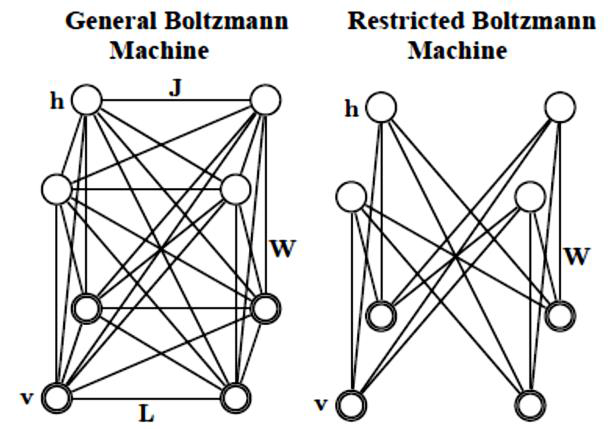
\includegraphics[width=6cm]{images/BM.png}
	 \end{column}
	 \begin{column}{0.5\textwidth}
		\begin{itemize}
		\item The top layer shows stochastic binary hidden units and the bottom layer shows stochastic binary visible units
		\item Some text comparing General BM
		\item In a Restricted Boltzmann Machine the joints between hidden units and also between visible units are disconnected
		\end{itemize}
	 \end{column}
	\end{columns} 
  \end{frame}
  \subsection{Restricted Boltzmann Machines}
  
  \begin{frame}
    \frametitle{Sample frame title}
    %\framesubtitle{A bit more information about this}
    Model of a Restricted Boltzmann Machine as a complete bipartite graph. Restricted Boltzmann Machine can be regarded as stochastic neural network, where the nodes and edges correspond to neurons and synaptic commections, respectively.
    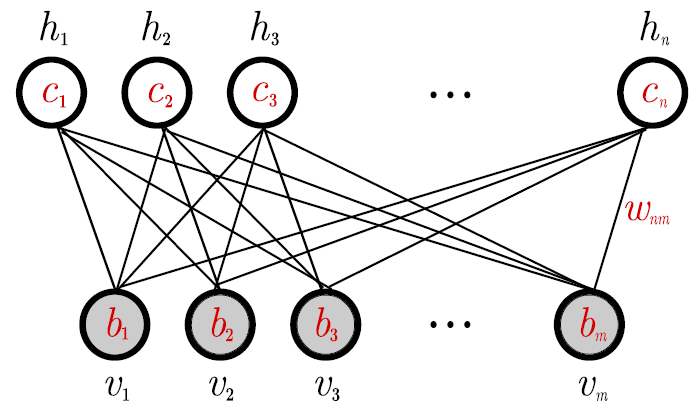
\includegraphics[width=8cm]{images/RBMnetworkGraph.png}
    \captionof{\TINY Figure}
			{\TINY The network graph of an RBM with n hidden and m visible units, Source: A.Fischer, Ch.Igel: Training Restricted Boltzmann Machines: An Introduction}
    
  \end{frame}
  \begin{frame}
  \frametitle{Some useful math equations}
  %Energy function
  \begin{align}
      \mathbf{E(v,h) = \sum_{i=1}^{V} \frac{(v_i - b_i^v)^2}{2\sigma_i^2} - \sum_{j=1}^{H} b_j^h h_j - \sum_{i=1}^{V} \sum_    {j=1}^{H} \frac{v_i}{\sigma_i} h_j w_ij}
  \end{align}

  %Probability of (v,h)
  \begin{align}
      \mathbf{p(v,h) = \frac{e^{-E(v,h)}}{\sum_x \sum_k e^{-E(x,k)}}}
  \end{align}
  \end{frame}
  
  \subsection{Contrastive Divergence} 
  \begin{frame}
  \frametitle{Contrastive Divergence with Gibbs sampling}
  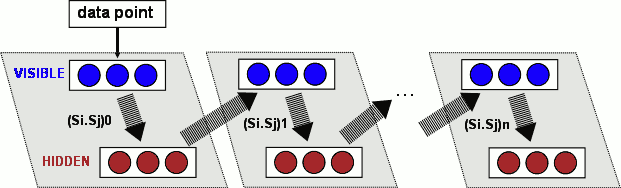
\includegraphics[width=8cm]{images/trainRBM.png}
  \end{frame}
  \section{Implementation}
  \begin{frame}
  \frametitle{Generative and Discriminative models of RBM}
  \begin{columns}
        \begin{column}{0.3\textwidth}
            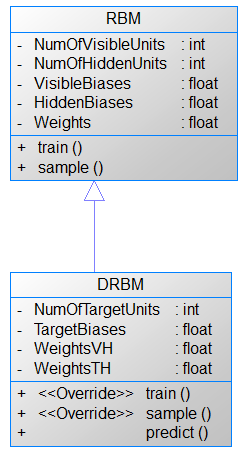
\includegraphics[width=3cm]{images/classDiagram.png}
        \end{column}
        \begin{column}{0.7\textwidth}
			\centering
			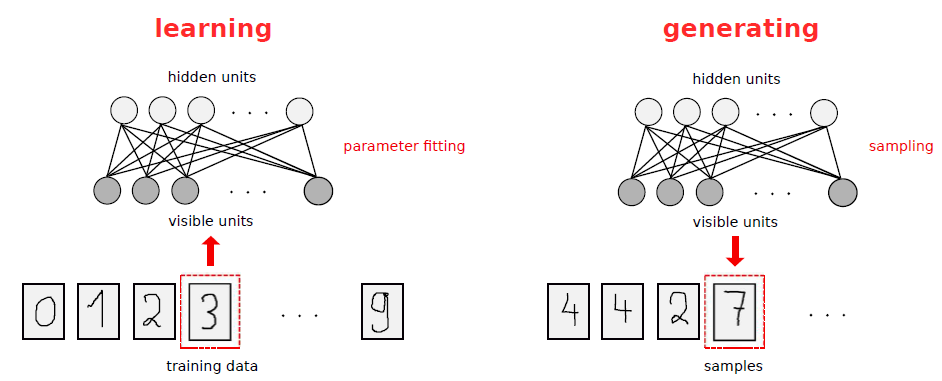
\includegraphics[width = 7cm]{images/generativeRBM.png}
			\captionof{\TINY GRBM}
			{\TINY Source: A.Fischer, Ch.Igel: Training Restricted Boltzmann Machines: An Introduction}
			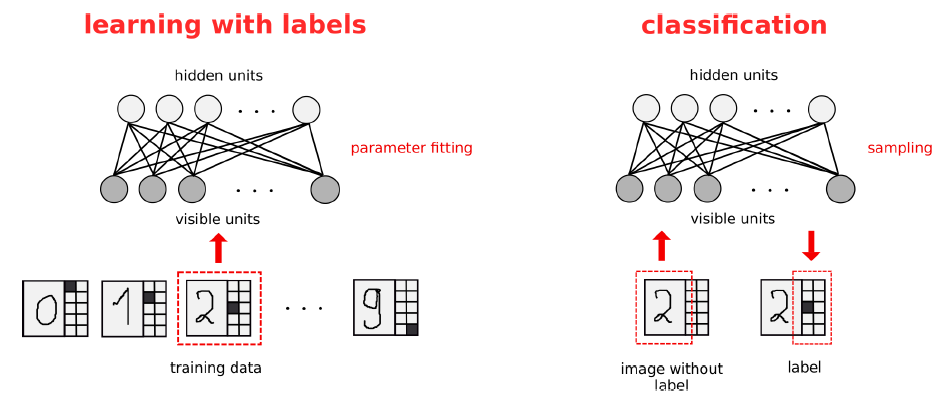
\includegraphics[width = 7cm]{images/DRBM.png}
			\captionof{\TINY DRBM}
			{\TINY Source: A.Fischer, Ch.Igel: Training Restricted Boltzmann Machines: An Introduction}
        \end{column}
    \end{columns}
  \end{frame}
   \begin{frame}
    \frametitle{Generative model}
    \begin{itemize}
	\item Train phase - fitting RBM parameters so that to model distribution of the training data 
	\item Training performed on inputs from user-given class
	\item Sample phase - trained RBM used to generate samples from learned distribution
	\item Shows reconstructed image for the user-specified digit
	\end{itemize}
	\end{frame}
  \begin{frame}
  \frametitle{RBM for classification}
  Training method:
  \begin{itemize}
	\item Models a joint distribution of inputs (x) and target classes (y)
	\item Has two sets of visible units and two weight matrices: between x and h (W) and between y and h (U)
	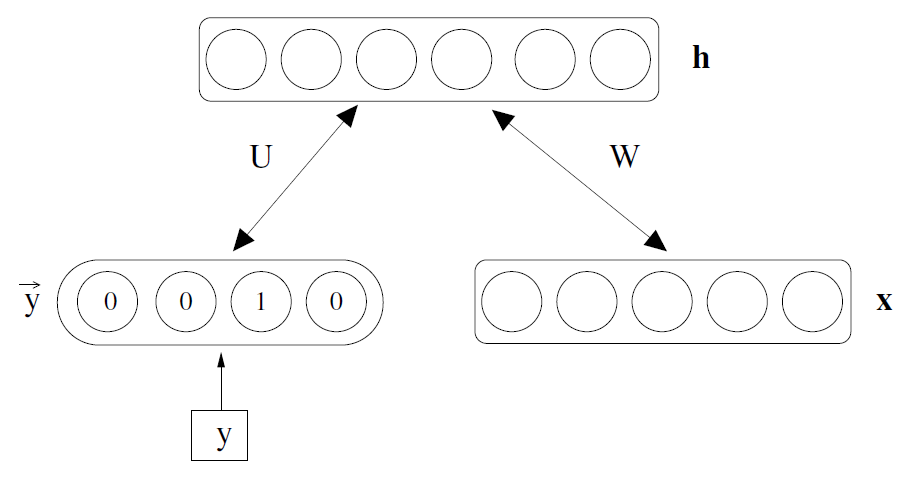
\includegraphics[width=5cm]{images/jointProbModel.png}
	\item Computes gradients for a mini-batch 
	\item Updates weights with mean gradients and user-defined learning rate
	\item Iterates through whole dataset in defined number of epochs
	%\item Computes mean squared error between data and reconstruction, per mini-batch, and per epoch
	\end{itemize}
  \end{frame}
  \begin{frame}
  \frametitle{RBM for classification}
  Prediction method:
  \begin{itemize}
	\item Fix the visible variables corresponding to the image
	\item Sample target variables corresponding to the labels in chosen number of iterations
	\item Return probabilities of each class 
	\item Choose the class with highest probability
	\item Perform for each datapoint in testset
	\item Compare with original labels
	\item Count wrong predictions and accuracy
	\end{itemize}
  \end{frame}
  \section{Results}
  \begin{frame}
  \frametitle{Testing methodology and assumptions}
  \begin{itemize}
	\item Tested dataset - MNIST - handwritten digit images (28x28 pixels = 784 features) and their labels (0..9)
	\item Dataset divided into training (50000), validation (10000) and test (10000) subsets 
	\item Reducing to binary problem(binarization threshold = 0.5)
	%\item Parameters possible to test: size of training set, size of test set, learning rate, momentum, l2 penaltization, number of steps for contrastive divergence, size of hidden units, initial weight distribution, number of epochs for training, number of iterations for sampling, error threshold for traning, random state
	\end{itemize}
  \end{frame}
  
  \begin{frame}[plain]
    \frametitle{Testing generative model}
    \begin{itemize}
	\item Experiments on different numbers of hidden units
	\item First image is original, next are for hidden units in size of: 200;300;400;500;700)
	\end{itemize}
	\begin{columns}
		\begin{column}{0.15\textwidth}
            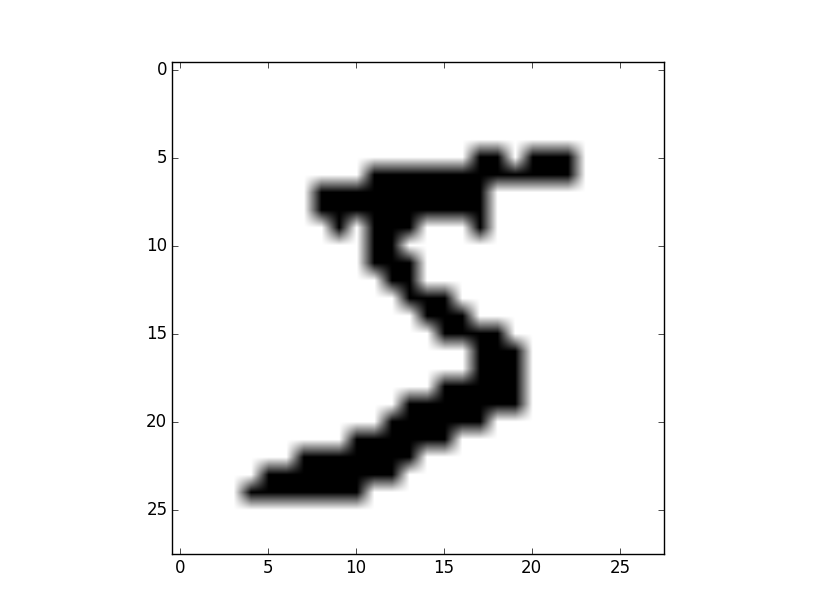
\includegraphics[width=2cm]{images/5original.png}
		\end{column}
		\begin{column}{0.15\textwidth}
			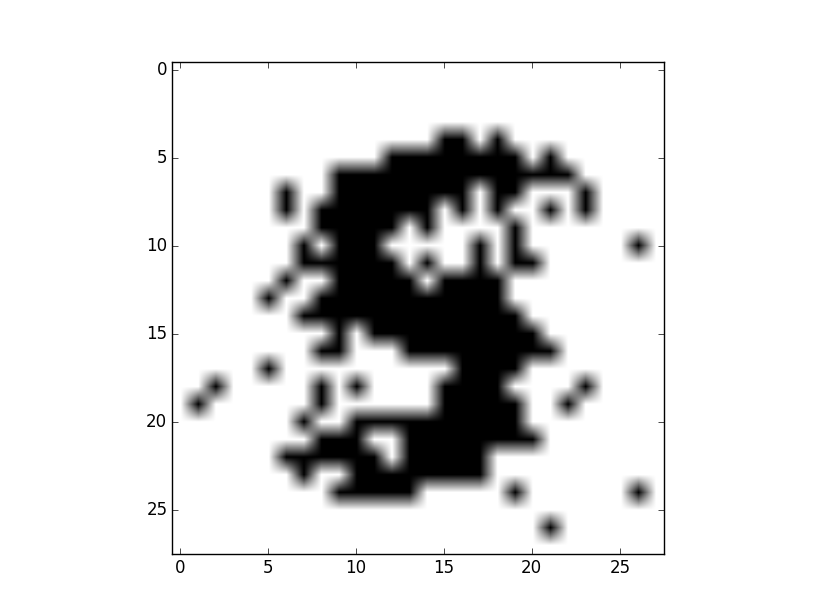
\includegraphics[width=2cm]{images/hidden200.png}
		\end{column}
		\begin{column}{0.15\textwidth}
			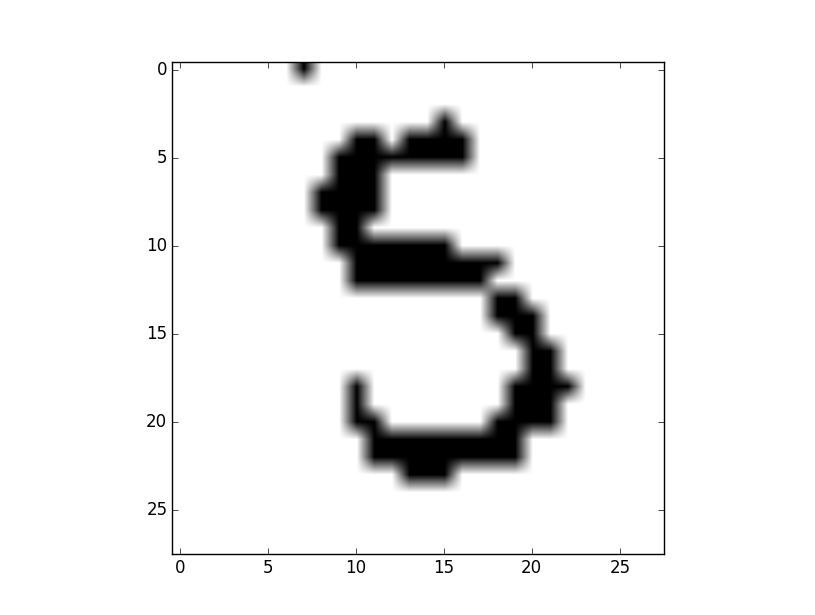
\includegraphics[width=2cm]{images/hidden300.png}
		\end{column}
		\begin{column}{0.15\textwidth}
			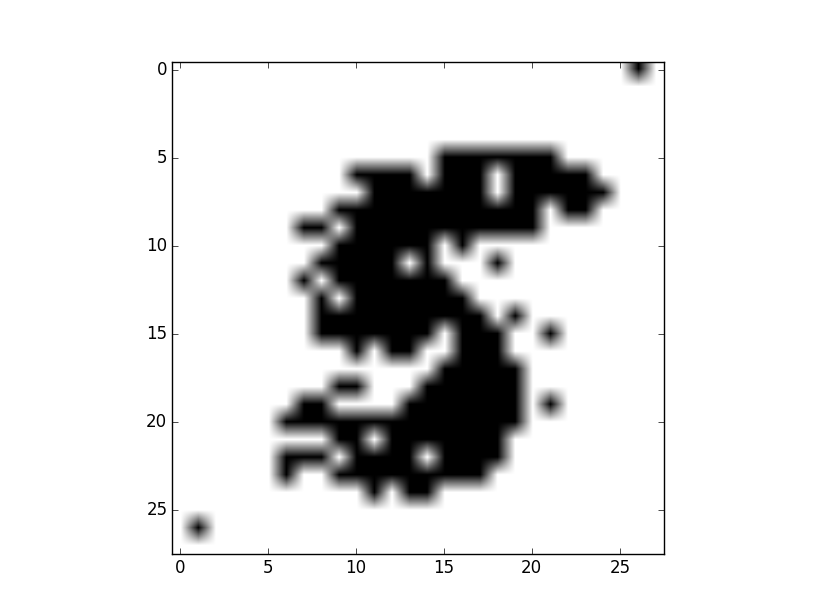
\includegraphics[width=2cm]{images/hidden400.png}
		\end{column}
		\begin{column}{0.15\textwidth}
			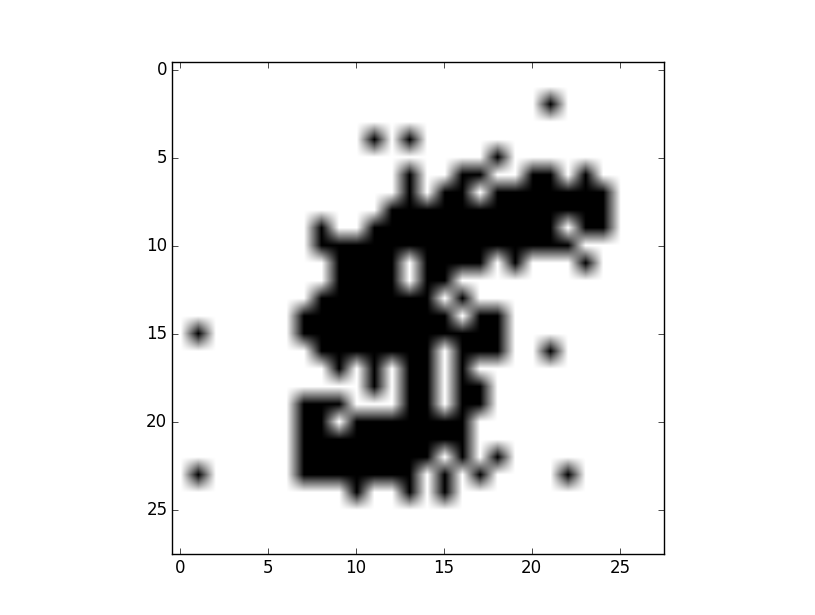
\includegraphics[width=2cm]{images/hidden500.png}
		\end{column}
		\begin{column}{0.15\textwidth}
			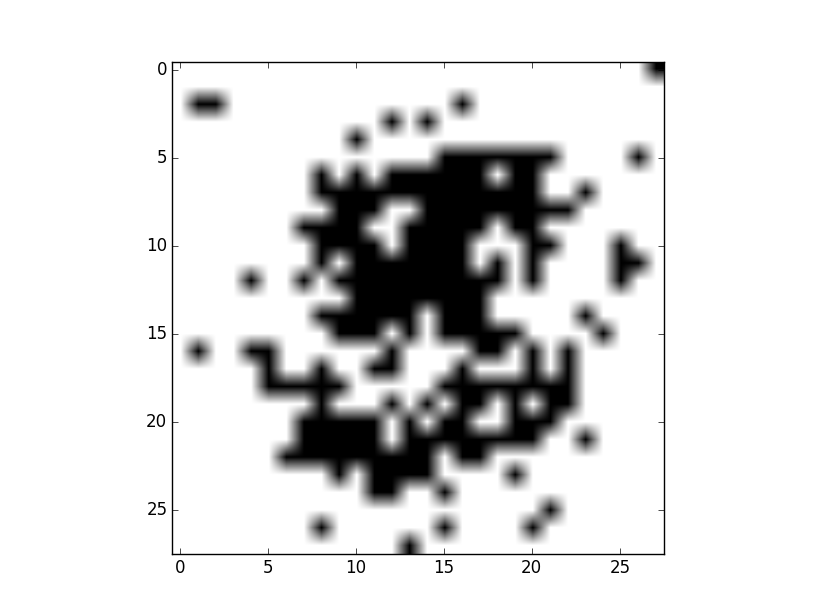
\includegraphics[width=2cm]{images/hidden700.png}
		\end{column}
    \end{columns}
    \begin{itemize}
    \item Generating "4": first image is original, next are for hidden units in size of: 100;200;300;400;500)
    \end{itemize}
    \begin{columns}
		\begin{column}{0.15\textwidth}
            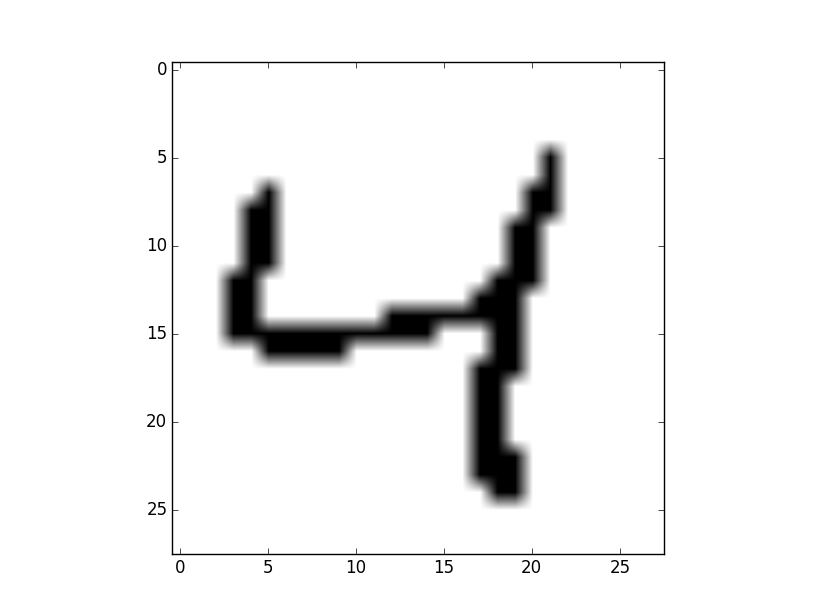
\includegraphics[width=2cm]{images/4original.png}
		\end{column}
		\begin{column}{0.15\textwidth}
			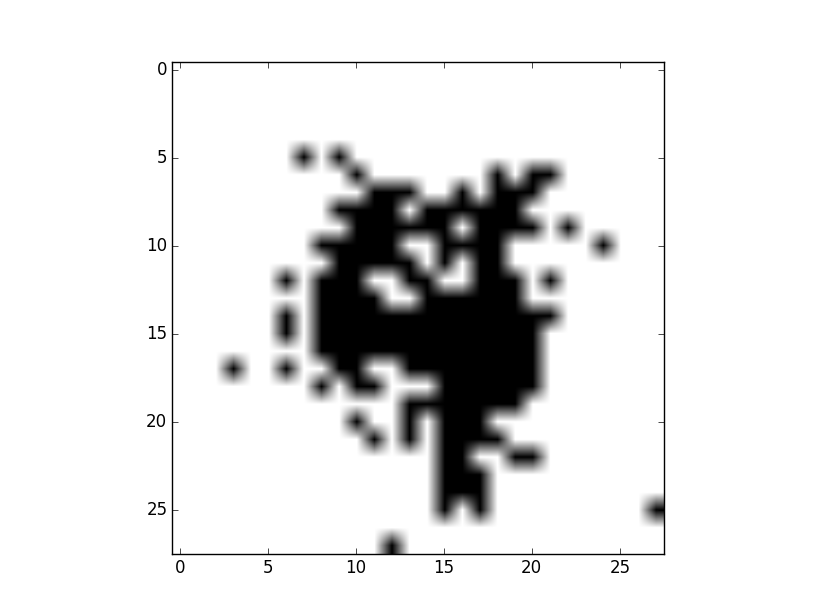
\includegraphics[width=2cm]{images/4Hidden100.png}
		\end{column}
		\begin{column}{0.15\textwidth}
			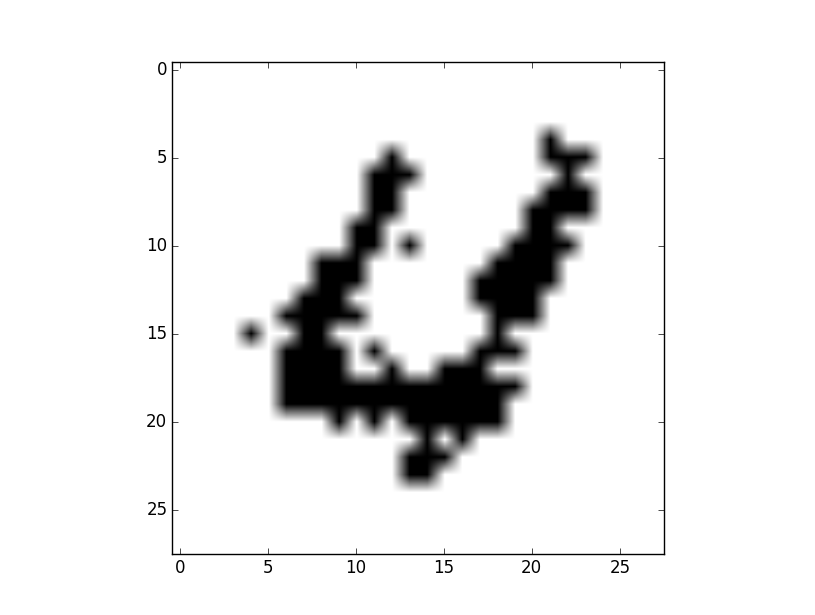
\includegraphics[width=2cm]{images/4Hidden200.png}
		\end{column}
		\begin{column}{0.15\textwidth}
			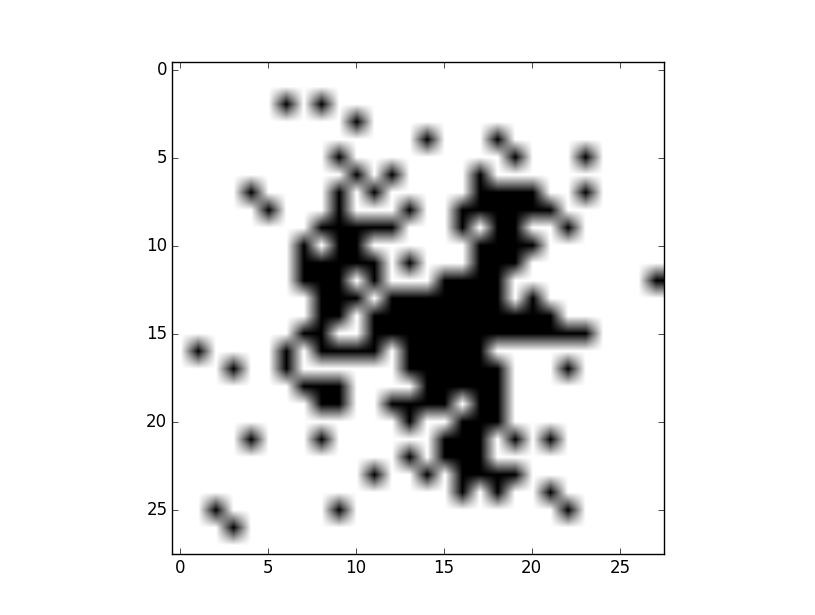
\includegraphics[width=2cm]{images/4Hidden300.png}
		\end{column}
		\begin{column}{0.15\textwidth}
			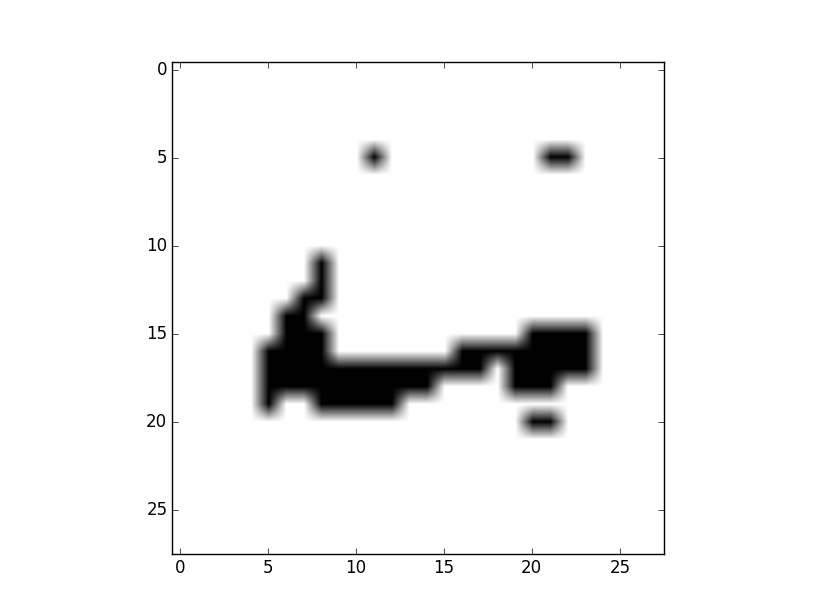
\includegraphics[width=2cm]{images/4Hidden400.png}
		\end{column}
		\begin{column}{0.15\textwidth}
			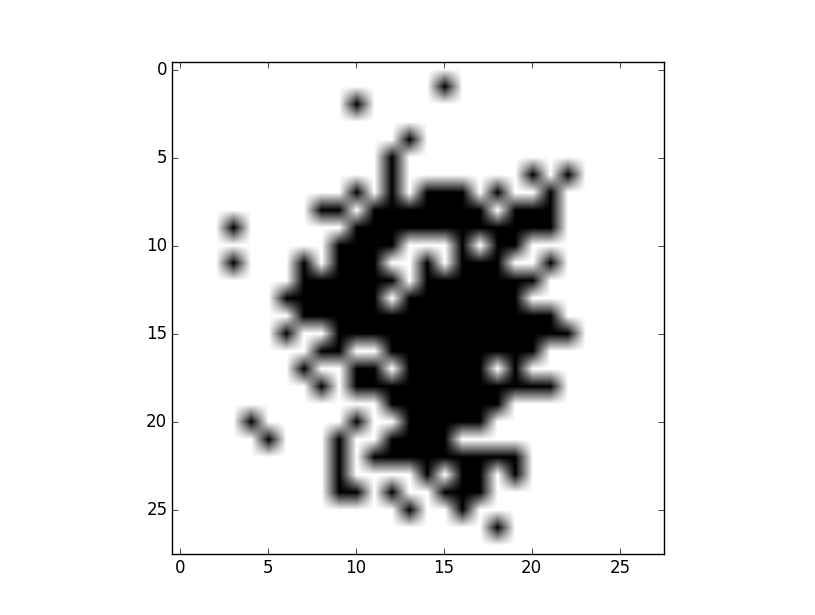
\includegraphics[width=2cm]{images/4Hidden500.png}
		\end{column}
    \end{columns}
    \begin{alertblock}{Remark}
	Different digit classes have different optimal hyperparameters
	\end{alertblock}
  \end{frame}
  \begin{frame}
    \frametitle{Testing generative model - joint-probabilities approach}
    \begin{itemize}
	\item Learning in mini-batches improved reconstruction and performance
	\item Momentum parameter for weight update other than 0.0 worsened results
	\item Optimized results for reconstruction after 500 epochs of training were very good (first is original, second with momentum=0.0, third with momentum=0.5):
	\end{itemize}
	\begin{columns}
		\begin{column}{0.3\textwidth}
            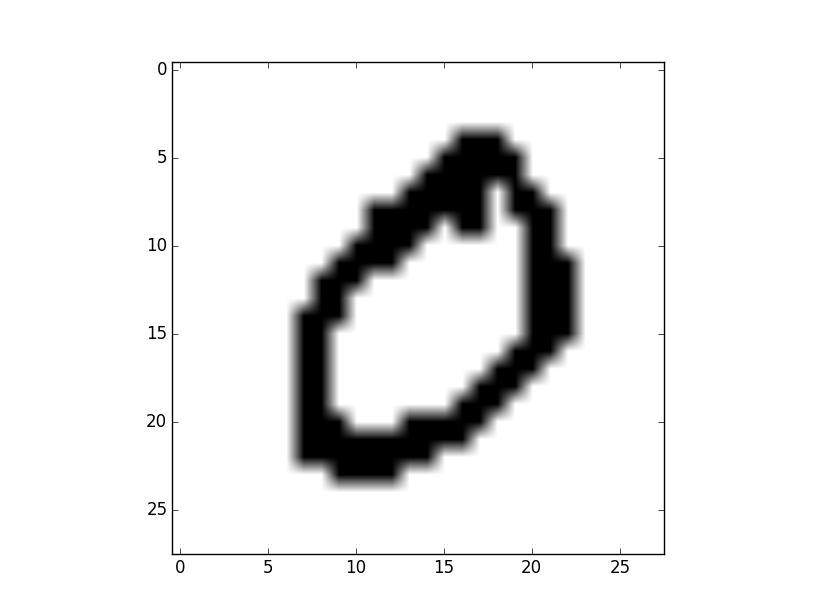
\includegraphics[width=3cm]{images/0original.png}
		\end{column}
		\begin{column}{0.3\textwidth}
			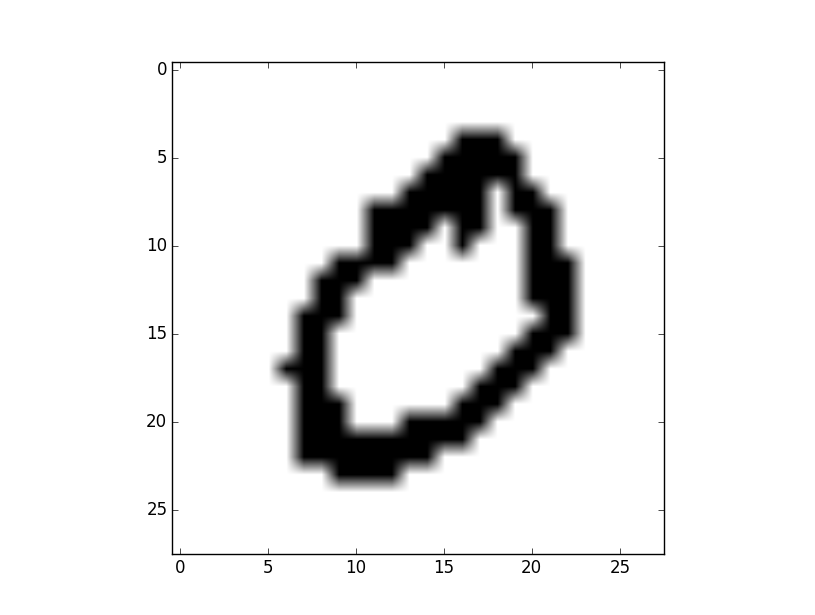
\includegraphics[width=3cm]{images/0_reconstructed_momentum00.png}
		\end{column}
		\begin{column}{0.3\textwidth}
			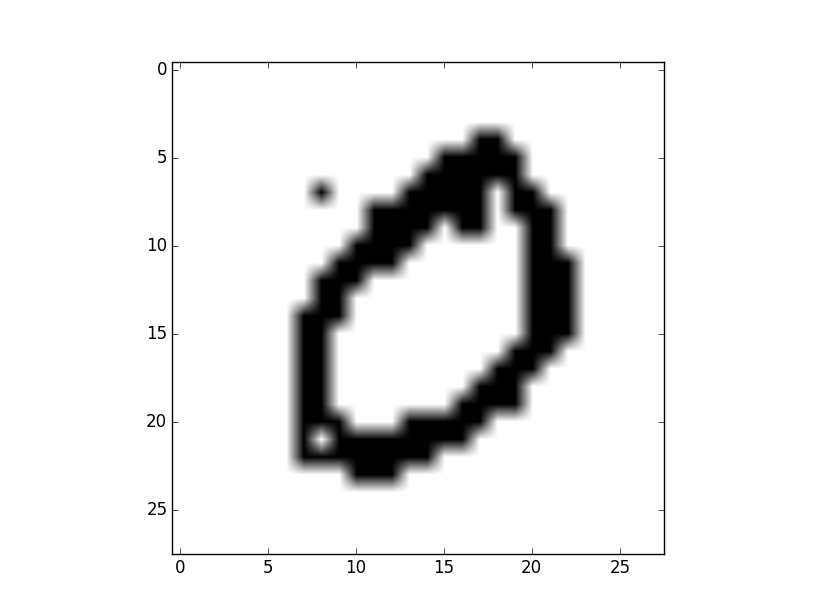
\includegraphics[width=3cm]{images/0_reconstructed_momentum05.png}
		\end{column}
    \end{columns}
    \begin{itemize}
    \item For 500-epoch training MSE falls below 1.0 - in about 30 minutes
    \end{itemize}
  \end{frame}
  \begin{frame}
  \frametitle{Monitoring progress of learning}
   Visualization of the weights of RBM (after 100. and 500. epoch)
   \begin{columns}
		\begin{column}{0.5\textwidth}
            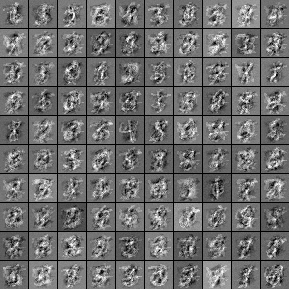
\includegraphics[width=5cm]{images/filtry_100epoch_50train.png}
		\end{column}
		\begin{column}{0.5\textwidth}
			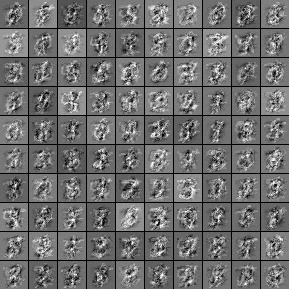
\includegraphics[width=5cm]{images/filters_epoch500_train50.png}
		\end{column}
    \end{columns}
    %Learned weights after 500 iterations on 50-train dataset  
  \end{frame}
  \begin{frame}[plain]
  \frametitle{Monitoring progress of learning}
  \framesubtitle{Reconstruction error for 100 epochs}
    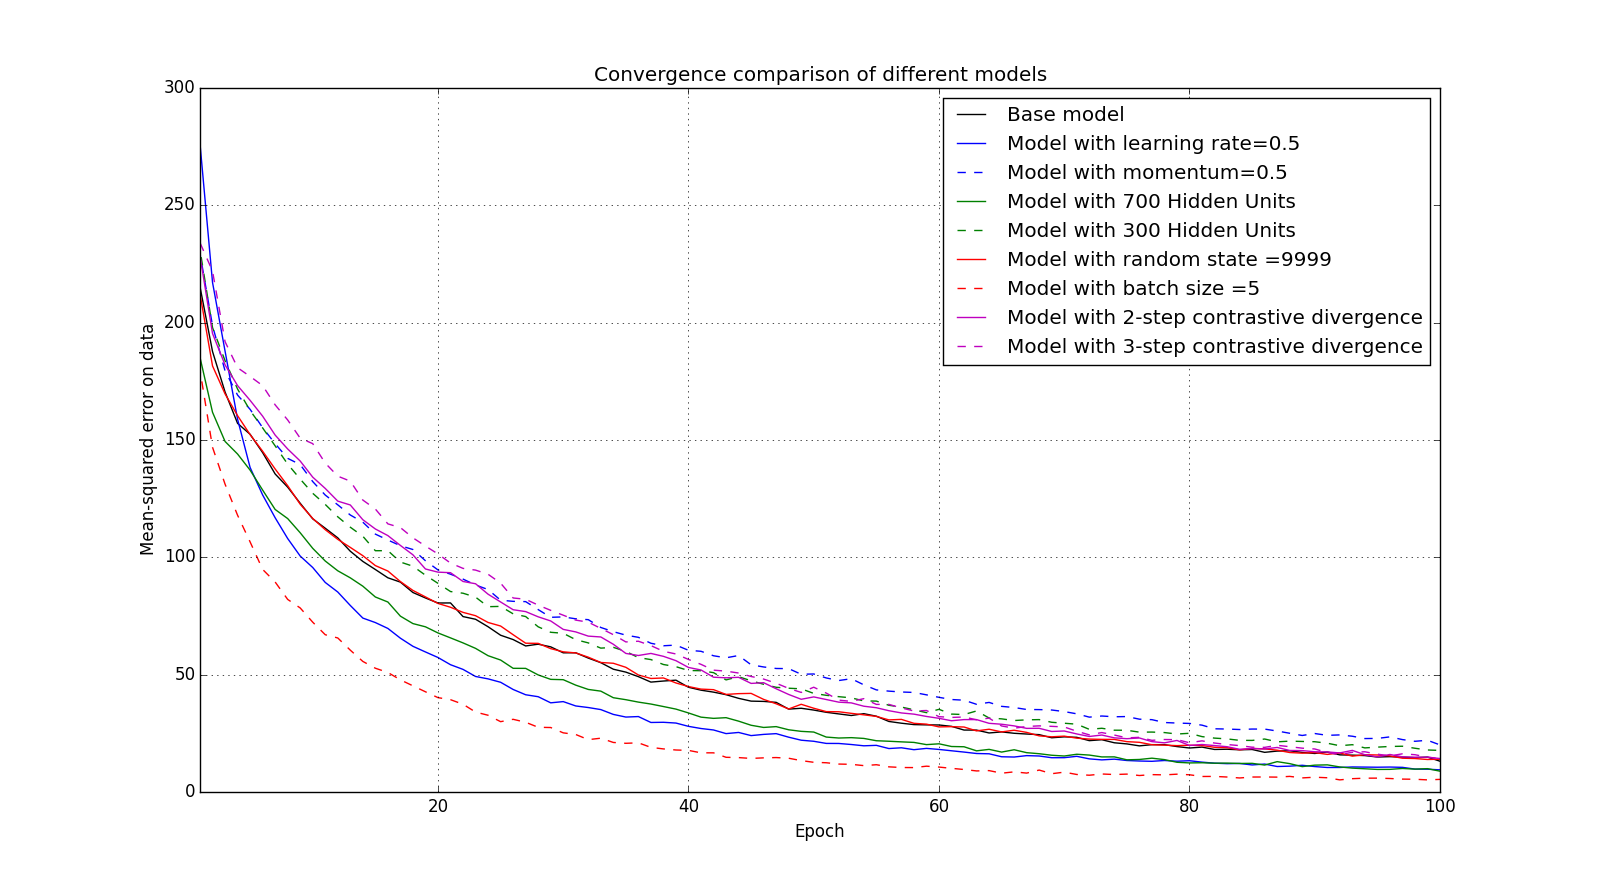
\includegraphics[width=10.5cm]{images/Plot_Convergence50train100epochs.png}
    \begin{alertblock}{Remark}
	The reconstruction error on the training set falls rapidly and consistently at the start of learning and then more slowly.
	\end{alertblock}
  \end{frame}
  \begin{frame}
  \frametitle{Model selection}
  \framesubtitle{Reconstruction error for first 10 epochs}
    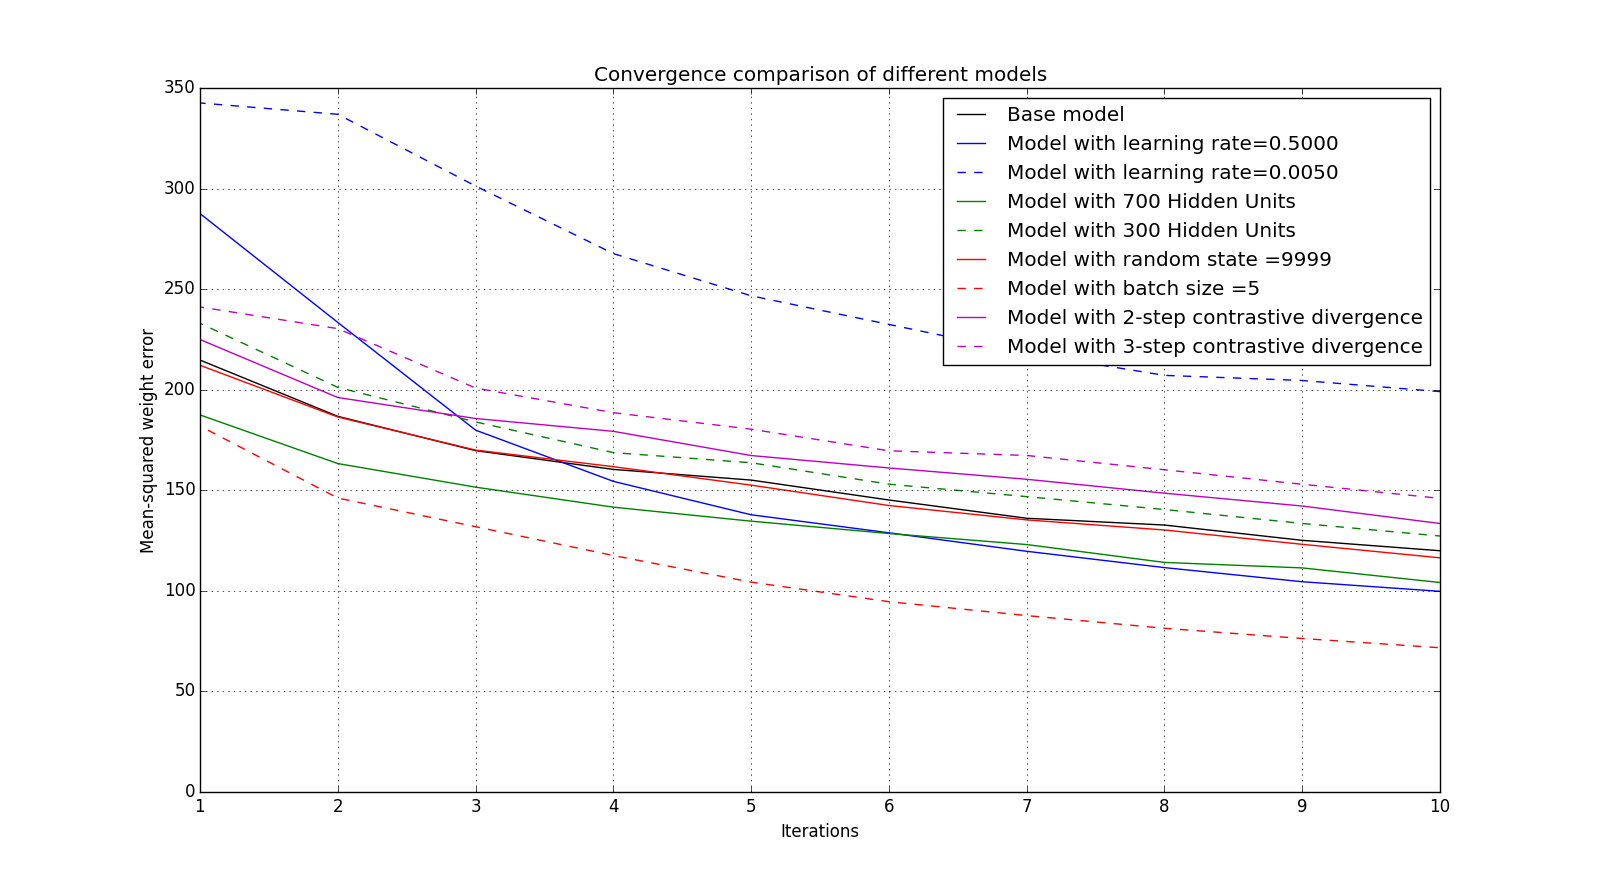
\includegraphics[width=12.5cm]{images/Plot_Convergence50train10epochs.png}
  \end{frame}
  \begin{frame}
  \frametitle{Model selection}
  \framesubtitle{Reconstruction error for last 5 epochs}
    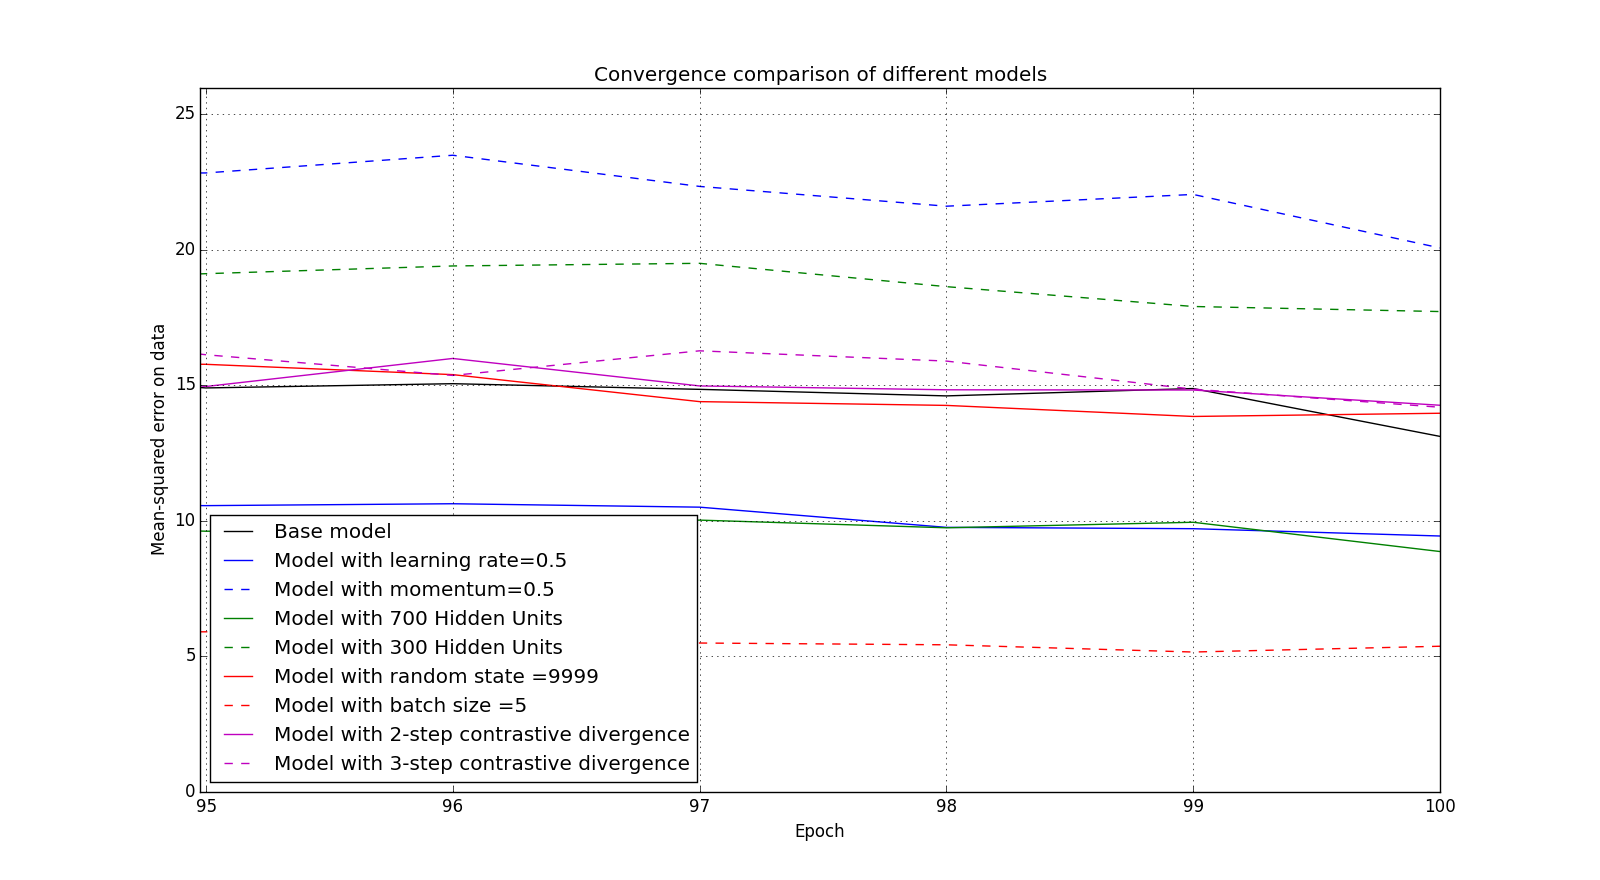
\includegraphics[width=12.5cm]{images/Plot_Convergence50train95-100epochs.png}
  \end{frame}
  \begin{frame}
    \frametitle{Model selection}
    \framesubtitle{Conclusions}
    \begin{itemize}
	\item Learning in smaller mini-batches and increasing number of hidden units (from 400 to 700) improved reconstruction
	\item However, these changes resulted in longer train time 
	\item Higher learning rate (0.5 instead of 0.05) caused reconstruction error to drop more sharply 
	\item Different random states do not change reconstruction error significantly
	\item 1-step contrastive divergence is optimal
	\end{itemize}
  \end{frame}
  \begin{frame}
    \frametitle{Testing RBM for prediction (I)}
    \begin{itemize}
    \item Optimal hyperparameters for training phase were chosen
	\item Performing 100 percent accurate classification on training data was trivial 
	\item Classification accuracy on test data achieved so far is 95 percent (MNIST 50000 trainset and 10000-testset)
	\item Better results are expected given greater computing power
	\end{itemize}
  \end{frame}
  \begin{frame}
    \frametitle{Testing RBM for prediction (II)}
    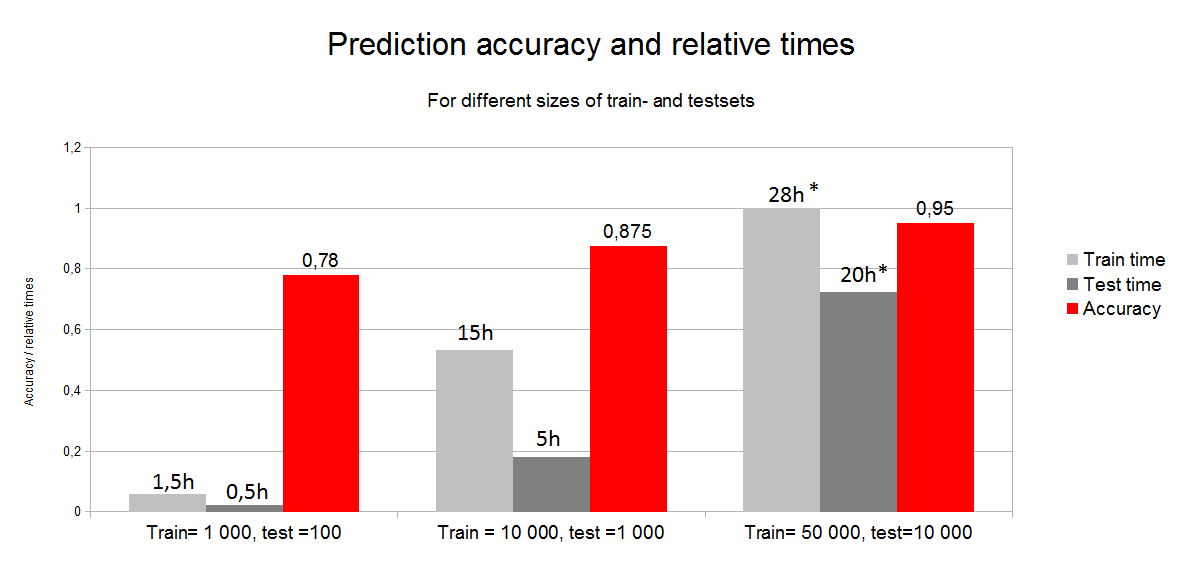
\includegraphics[width=9.5cm]{images/acc.png}
    \begin{itemize}
	\item Improving prediction accuracy on test data requires training a model on greater number of data input and sampling on greater number of test data inputs, but times are prohibitive for personal computing
	\end{itemize}
  \end{frame}
  \begin{frame}
    \frametitle{Plans for further work}
    \begin{itemize}
    \item Test-against-all-labels prediction approach
    \item Optimizing algorithms for best performance
	\item Testing on gaussian values
	\item Another dataset, possibly CIFAR
	\end{itemize}
  \end{frame}
  \begin{frame}[allowframebreaks]
  \frametitle<presentation>{Literature}    
  \begin{thebibliography}{10}    
  %\beamertemplatebookbibitems
  %\bibitem{Autor1990}
    %A.~Autor.
    %\newblock {\em Introduction to Giving Presentations}.
    %\newblock Klein-Verlag, 1990.
  \beamertemplatearticlebibitems
  \bibitem{Larochelle}
    Hugo Larochelle, Yoshua Bengio.
    \newblock Classification using Discriminative Restricted Boltzmann Machines.
    \newblock {\em Proceedings of the 25th International Conference on Machine Learning}, 2008.
   \bibitem{Hinton}
    Geoffrey Hinton.
    \newblock A Pratical Guide to Training Restricted Boltzmann Machines.
    \newblock {\em UTML TR 2010-003}, 2010.
   \bibitem{Fischer}
    Asja Fischer, Christian Igel.
    \newblock Training Restricted Boltzmann Machines: An Introduction.
    \newblock {\em UTML TR 2010-003}, 2(1):50--100, 2008.
  \end{thebibliography}
  \end{frame}
  \begin{frame}[plain]
  \frametitle{Questions?}
  \end{frame}
\end{document}
